\section*{Duchamp e Tarsila}
\autoria{Celestino B. Neto}
\avisoTextoForms

Li com alegria o texto apócrifo recém publicado no BOLETIME, onde um anônimo especula sobre a ideia de um parentesco entre Arte e Matemática. É importante que haja porosidade entre o universo das “humanas” e o das “exatas”.

Assim como um de nós, que estude matemática, poderia se insurgir com a afirmação de que “não existe muita diferença entre números racionais e números reais, pois ambos podem ter vírgulas seguidas de vários números”, alguém, com algum conhecimento na área de “humanas”, poderia se incomodar com generalizações, ainda que bem intencionadas, nas áreas da literatura, e das artes plásticas.

\begin{displayquote}
    \textit{\textbf{``...Malgré ses affinités avec Dada ou les surréalistes, Duchamp reste un artiste indépendant...''}}[1]
\end{displayquote}

Marcel Duchamp, artista independente, que flertou com diversos movimentos artísticos (dadaismo, fauvismo e cubismo), foi quem introduziu os “ready made” [2] no universo das artes plásticas . A “Roda de bicicleta”, criada em 1913 [3] foi sua primeira manifestação. A proposta do artista era deslocar “\textbf{objetos comuns, com ou sem modificações mínimas, para dentro de espaços museológicos}” [4], com o intento de se aproximar do conceito de indiferença visual. Isso liberaria o artista do império da “arte retiniana”, aquela voltada ao deleite visual, convidando, por outro lado, os apreciadores a uma reflexão sobre a linguagem da arte, o que abriu a via para a consolidação da ideia de arte como conceito [5].

Assim, a obra “Roda de bicicleta”, no contexto em que se inseria, não se vincula à discussão utilidade/inutilidade de um determinado objeto, como insinua o texto apócrifo publicado. Não está aí o compromisso do fazer artístico. “\textbf{Duchamp... mostrou a obra de arte pronta [6] como um subproduto, resultado de uma “digestão” artística. A partir da intervenção do artista, o objeto, agora um trabalho artístico, incorpora um valor cultural.}” [7].

\begin{figure}[H]
    \centering
    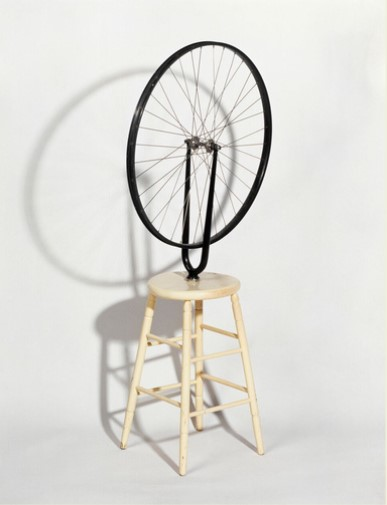
\includegraphics[width=0.65\linewidth]{textos/img/duchamp_a_roda_de_bicicleta.jpg}
    \\
    \legendaFigura{1}{\textit{A Roda de Bicicleta, Marcel Duchamp}}
\end{figure}

Já o “Abaporu”, de Tarsila do Amaral, foi concebido como presente ao seu então marido, o escritor Oswald de Andrade, que ao recebê-lo nomeou (junto ao poeta Raul Bopp) a obra à partir de vocábulos da língua tupi que significam “homem que come gente”, criando assim um vínculo com o Movimento Antropofágico “que se propunha a deglutir a cultura estrangeira e adaptá-la ao Brasil” [8].

Insinua o texto apócrifo, que Tarsila teria tido a intenção de retratar um Abaporu [9]. Sabe-se que esta obra, ícone do modernismo brasileiro, “através do emprego de cores puras, das linhas simples, da captação sintética, sentimental e ingênua da realidade brasileira” [10], nos passava uma mensagem plástica regionalista (brasileira), cujo conteúdo foi desvelado posteriormente por Oswald.

\begin{figure}[H]
    \centering
    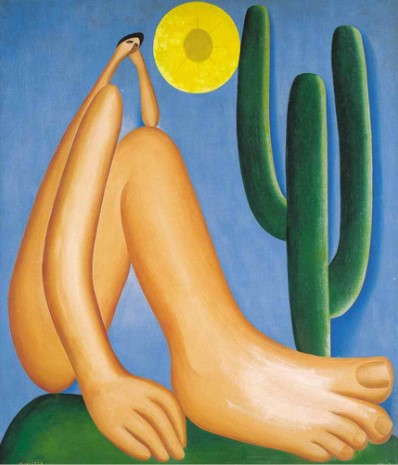
\includegraphics[width=0.65\linewidth]{textos/img/tarsila_abaporu.jpg}
    \\
    \legendaFigura{1}{\textit{Abaporu, de Tarsila do Amaral}}
\end{figure}

Foi feliz a escolha de Duchamp e de Tarsila no texto apócrifo, dois marcos que são na produção artística do séc.XX, assim como a tentativa de inserção de elementos não matemáticos no ambiente do IME, como forma de alargar a visão limitada do mundo que somos levados a nutrir, em função da falta de tempo que a grade curricular nos impõe. Fica então uma sugestão: mais rigor nos “axiomas” que escolhemos ao fazer a “demonstração de um teorema” não matemático, se me permitirem esta transposição.

O mesmo rigor empregado no fazer da Matemática precisa ser valorizado na produção de textos e no uso da língua, no ambiente da Matemática, para que aquilo que escrevemos tenha recepção adequada e relevante nos ambientes acadêmicos menos afeitos aos números, mas absolutamente comprometidos com o rigor das proposições.

\emph{\textbf{Sobre o autor:} Celestino Neto cursa atualmente, no IME- USP, o terceiro semestre de licenciatura em Matemática (noturno), é arquiteto formado pela FAU-USP e bacharel em Letras com habilitação em Português e Linguística pela FFLCH-USP.}

\vfill % para grudar no fim da página

\textbf{[1]} \emph{Tradução livre: “...Apesar de afinidades com Dada ou os surrealistas, Duchamp continua sendo um artista independente”}
\\
\textbf{[2]} \emph{Tradução livre: “obra de arte pronta”}
\\
\textbf{[3]} E não em 1951 como informa o texto apócrifo.
\\
\textbf{[4]} \emph{Ready Made: Inclusão Ruidosa}; PELED, Yiftah, pg. 1724
\\
\textbf{[5]} Enciclopédia Britannica para “Conceptual art”. \emph{Tradução livre: “arte conceitual tem sido descrita como um dos movimentos mais influentes do final do sécXX, uma extensão lógica do trabalho iniciado pelo artista francês Marcel Duchamp em 1914 para quebrar a primazia do perceptivo em arte.”}
\\
\textbf{[6]} “ready made”
\\
\textbf{[7]} Ready Made: Inclusão Ruidosa; PELED, Yiftah, pg. 1727
\\
\textbf{[8]} Programa de pos-graduação em artes visuais da UFBA
\\
\textbf{[9]} “O Abaporu jamais foi visto em qualquer lugar, por mais remoto que seja, mas ainda assim Tarsila do Amaral foi capaz de retratá-lo”
\\
\textbf{[10]} Abaporu e a “invenção” da arte brasileira; SILVA, Dalmo de Oliveira Souza e, pg. 540